The entirety of our work is based on the SGD framework described in section \ref{sec:sgd}. In particular we insisted on three phases of the algorithm, namely the initialization, the choice of the descent direction and the step size. We show that the initialization play a crucial role in the learning process and can, alone, dictate if the learning process will be "successful"\footnote{Here we refer to artificial task where a criterion for success is easily defined.} or not. We than propose a strategy to choose a descent direction which helps to deal with the vanishing gradient. As for the learning rate we use a technique which is entirely equivalent to the gradient clipping trick described and used in \cite{pascanu}.

\section{Notation}
Before focusing on each phase we will introduce some notation which we will need in the following sections.

Consider a loss function $g$ for some time step $\tau$. Defining 
\begin{equation}
\nabla_{\mat{W_{rec}}} g_{|k}  \defeq \frac{\partial g}{\partial \vec{a}^{\tau}} \cdot \frac{\partial \vec{a}^{\tau}}{\partial \vec{a}^k} \cdot \frac{\partial^+ \vec{a}^k}{\partial \mat{W}^{rec}},
\end{equation}
and recalling the results of section \ref{sec:rnn_grad} we have
\begin{equation}
	\frac{\partial g_{\tau}}{\partial \mat{W}^{rec}} = \sum_{k=1}^{\tau} \nabla_{\mat{W_{rec}}} g_{|k}.
\end{equation}
We refer to $\nabla_{\vec{x}} g_{|k}$ as temporal gradient for time step $k$ w.r.t. the variable $\vec{x}$ and is easy to see that it is the gradient computed imagining to replicate variable $\vec{x}$ for each time step and taking the derivatives w.r.t. the variable for the step $k$.

The \textbf{vanishing gradient} problem appears then, under this new notation, when the norm of the temporal components $\nabla_{\vec{x}} g_{|k}$ are exponentially bigger for more recent time steps.

\section{Initialization}
The first moment of the learning process is the initialization of the variables. We found that the choice of the initial value for the recurrent matrix $\mat{W_rec}$ has a big impact on the entire learning process. Recall the results from section  \ref{sec:vanishing} where we saw that too small singular values of such matrix are a sufficient condition for the gradient to vanish. Although a sufficient condition that guarantees the gradient not to vanish is not known, the results on the singular values encourage to explore initialization techniques with higher singular values and more in general spectral radius of the recurrent matrix. A similar suggestion, motivated by other consideration was given in the ESN field \cite{reservoirSummary}.

We initialize the recurrent matrix sampling from a gaussian distribution of zero mean and variance equal to 0.1 and then scaling the matrix to have a specified spectral radius. In figure \ref{fig:temporal_norms} we show the temporal components w.r.t. all the variables of the model varying the spectral radius in [0.8, 0.9, 1, 1.1, 1.2] computed on a hundred samples for the temporal order task.

\begin{figure}
    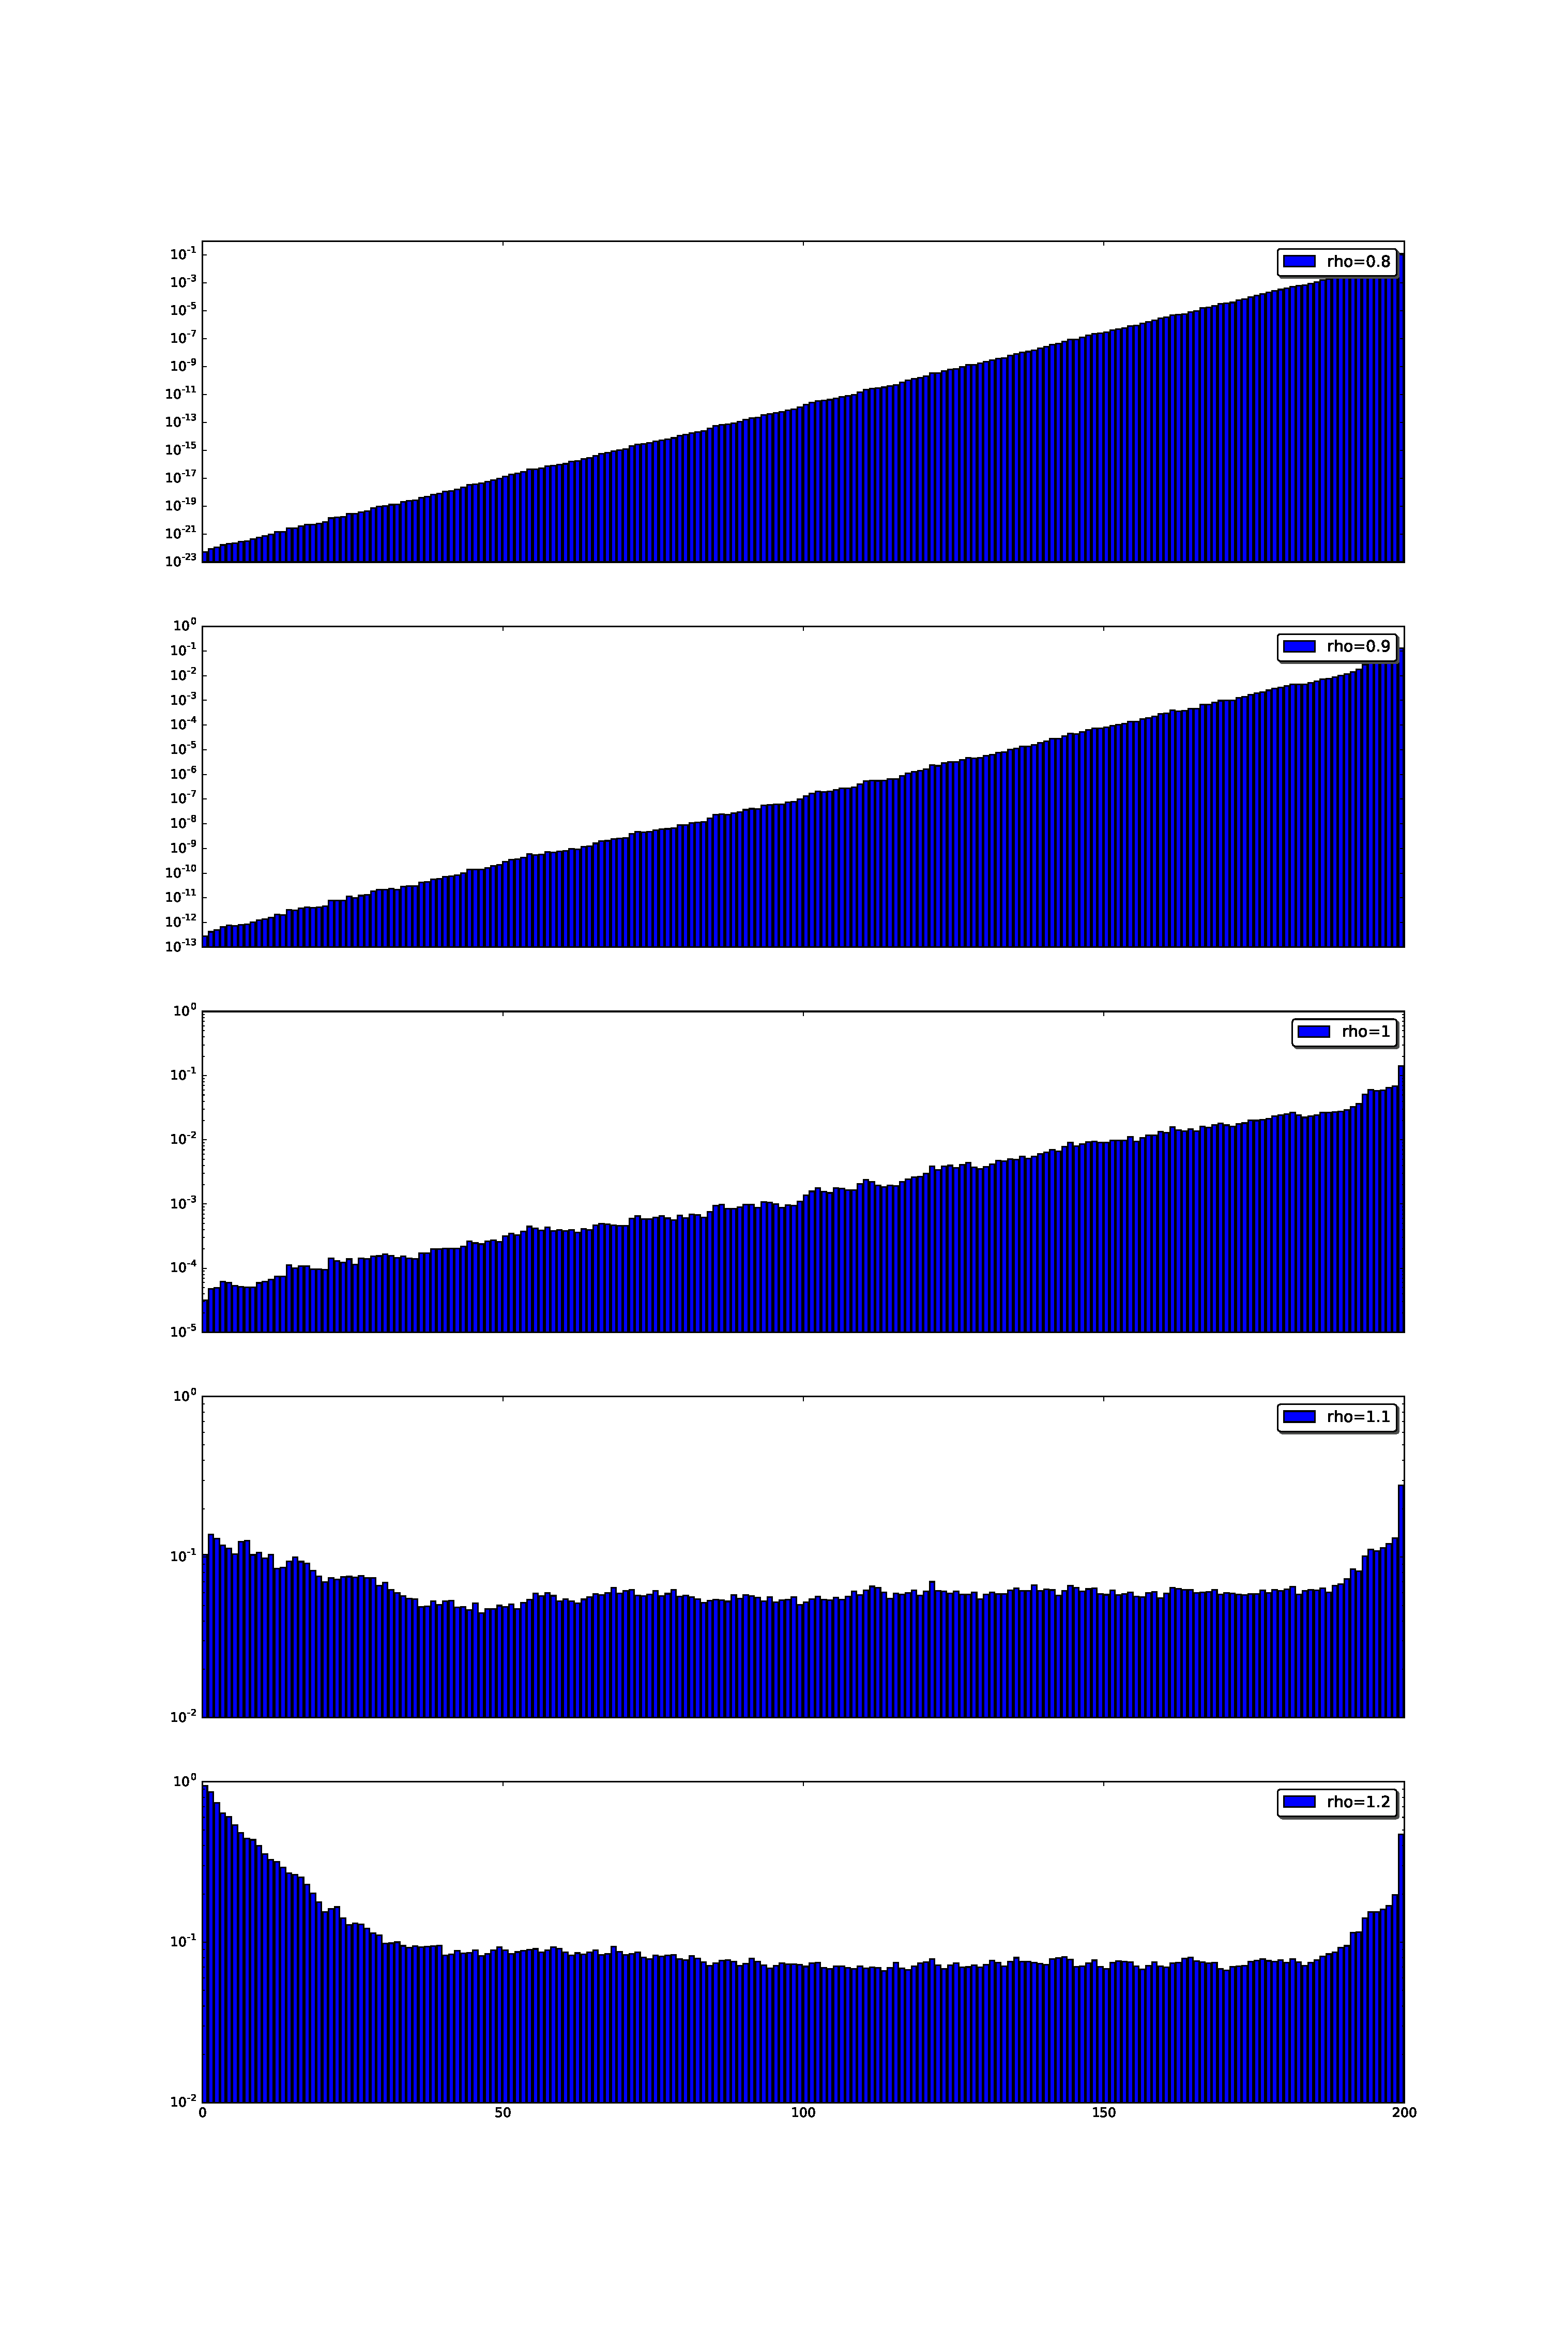
\includegraphics[width=0.9\textwidth]{chapter3/temporal_components.eps}
    \caption{Temporal components for the temporal order task varying the spectral radius of the recurrent matrix. y axis is in logarithmic scale.}
    \label{fig:temporal_norms}
\end{figure}

The first two cases, the one with spectral radius less than one, are perfect example of vanishing gradient instances: more recent temporal components have norm exponentially bigger than the more distant ones (please note that the y axis is in logarithmic scale). On the contrary such phenomenon is not observed in the cases of spectral radius bigger than one where the temporal components have roughly the same norm.

This evidence suggest 
\\
EXPERIMENTS HERE ?

\section{Descent direction}

The idea is to use the structure of the gradient to compute a "descent" direction which does not suffer from the vanishing problem.
\begin{itemize}
	\item normalize the temporal components:
	\begin{equation}
	g_t(\vec{x}) = \frac{\nabla L_{|t}(\vec{x})}{\norm{\nabla L_{|t}(\vec{x})}}.
	\end{equation}
	
	\item combine the normalized gradients in a simplex:
	\begin{equation}
	g(\vec{x}) = \sum_{t=1}^T \beta_t \cdot g_t(\vec{x}).
	\end{equation}
	
	with $\sum_{t=1}^T\beta_t=1, \beta_t>0$ (randomly picked at each iteration).
	\item exploit the gradient norm:
	\begin{equation}
	d(\vec{x}) = \norm{\nabla L (\vec{x})}\frac{g(\vec{x})}{\norm{g(\vec{x})}}.
	\end{equation}
\end{itemize}
\section{Learning rate}

Given a direction $\vec{d}_k$ the step $\alpha_k$ is chosen as:

\begin{equation}
\alpha_k = 
\begin{cases}
	\mu \quad &\mbox{if} \norm{\vec{d}_k}_2 \leq c\\
	\frac{\mu}{\norm{\vec{d}_k}_2} \quad & otherwise
\end{cases},
\end{equation}
where $\mu$ and $c$ are some positive constants. The idea is to use a constant step when the direction has an enough small norm and vice-versa choose a step which inversely proportional when such norm is too big. The idea is that, if the descent direction has a too big norm we might take a too big step. This technique is know as \textit{gradient clipping} and has been used for RNNs training (with first oder methods) in \cite{pascanu} and \cite{mikolov}. We confirm, as found in these works, that this trick is essential for RNNs training where, considering the anti-gradient descent direction, we deal with fast changing norms.
\section{Proof of convergence}
 
\documentclass{article}
\usepackage[utf8]{inputenc}
\usepackage[italian]{babel}
\usepackage{graphicx}
\usepackage{cite}
\usepackage[hidelinks]{hyperref}
\usepackage{listings}
\usepackage{latexsym}
\usepackage{amsmath}
\usepackage{proof}
\usepackage{stmaryrd}
\usepackage{amssymb}
\usepackage{epstopdf}
\usepackage{pgf}
\usepackage{tikz}
\usepackage[noend]{algpseudocode}
\usepackage[ruled,noline,linesnumbered]{algorithm2e}
\usetikzlibrary{automata,arrows}
\let\emptyset\varnothing

\graphicspath{ {./images/} }

%%Notation:

%%vectors
\renewcommand{\vec}[1]{\boldsymbol{#1}}
%%sets
\newcommand{\set}[1]{\mathcal{#1}}
%%matrixes
\newcommand{\mat}[1]{#1}
%%norm
\newcommand{\norm}[1]{\left\Vert #1 \right\Vert}
%%defeq
\newcommand{\defeq}{\triangleq}
%%
\newcommand{\net}[1]{\mathrm{#1}}
%% pair<x,y>
\newcommand{\pair}[2]{\langle#1,#2\rangle}

\title{Stochastic gradient descent}
\author{Giulio Galvan}

\begin{document}
	\maketitle
\noindent
Consider the stochastic optimization problem 
\begin{equation}
	\underset{\vec{x} \in \mathbb{R}^n}{\text{min}} f(\vec{x}) = \mathbb{E[F(\vec{x}, \vec{\xi})]},
	\label{eq:stochastic_prob}
\end{equation}
where $\vec{\xi} \in \Omega \subset \mathbb{R}^d$ is a random vector.
Suppose $f(\cdot)$ is continuous, strongly convex (with constant $c$) and there exists a compact level set of $f(\cdot)$, hence (\ref{eq:stochastic_prob}) has a unique optimal solution $\vec{x}_*$. Let also $L$ be the Lipschitz constant of $\nabla f$.
We make the following two assumptions:
\begin{itemize}
	\item	It is possible to generate independent identically distributed samples of $\vec{\xi}$
	\item There exists an oracle which, for a given point $(\vec{x}, \vec{\xi})$ return a stochastic descent direction $D(\vec{x}, \vec{\xi})$ such that $d(\vec{x})\defeq\mathbb{E}[D(\vec{x}, \vec{\xi})]$ satisfies:
	\begin{equation}
	-(\vec{x}-\vec{x}_*)^T (\nabla f(\vec{x}) -g(\vec{x})) \geq -\mu L \norm{\vec{x}_j-\vec{x}_*}^2_2\quad \forall \vec{x} \in \mathbb{R}^n,
	\label{eq:angular_condition}
	\end{equation}
	for some $\mu \in (0,\frac{c}{L}) $.
\end{itemize}
Consider the algorithm defined by
\begin{equation}
	\vec{x}_{j+1} = \vec{x}_j -\gamma_j D(\vec{x}_j,\vec{\xi}_j).
	\label{eq:stochastic_algo}
\end{equation}
Each iterate $\vec{x}_j$ of such random process is a function of the history $\vec{\xi}_{[j-1]}=(\vec{\xi}_1,\dots, \vec{\xi}_{j-1})$

Let $A_j\defeq \norm{\vec{x}_j-\vec{x}_*}^2_2$ and $a_j\defeq\mathbb{E}[A_j]$.
From (\ref*{eq:stochastic_algo}) we get
\begin{equation}
\begin{aligned}
	A_{j+1} &= \frac{1}{2}\norm{\vec{x}_j - \gamma_jD(\vec{x}_j,\vec{\xi}_j) -\vec{x}_*}^2_2\\ 
	&= A_j +\frac{1}{2}\gamma_j^2\norm{D(\vec{x}_j,\vec{\xi}_j)}^2_2 - \gamma_j(\vec{x}_j-\vec{x}_*)^TD(\vec{x}_j,\vec{\xi}_j).
\end{aligned}
\label{eq:aj_rec}
\end{equation}
Since $\vec{x}_j = \vec{x}_j(\vec{\xi_{[j-1]}})$ is independent of $\vec{\xi}_j$ we have
\begin{equation}
\begin{aligned}
	\mathbb{E}_{\vec{\xi}_{[j]}}[(\vec{x}_j-\vec{x}_*)^TD(\vec{x}_j,\vec{\xi}_j)] &= \mathbb{E}_{\vec{\xi}_{[j-1]}}[\mathbb{E}_{\vec{\xi}_{[j]}}[(\vec{x}_j-\vec{x}_*)^TD(\vec{x}_j,\vec{\xi}_j)]|\vec{\xi}_{[j-1]}]\\
	&= \mathbb{E}_{\vec{\xi}_{[j-1]}}[(\vec{x}_j-\vec{x}_*)^T\mathbb{E}{\vec{\xi}_{[j]}}[D(\vec{x}_j,\vec{\xi}_j)]|\vec{\xi}_{[j-1]}]\\
	&=\mathbb{E}_{\vec{\xi}_{[j-1]}}[(\vec{x}_j-\vec{x}_*)^Td(\vec{x}_j)]\\
\end{aligned}
\label{eq:independece}
\end{equation}
Let now assume that there exists $M>0$ such that
\begin{equation}
	\mathbb{E}[\norm{D(\vec{x},\vec{\xi})}^2_2]\leq M^2 \quad \forall \vec{x} \in \mathbb{R}^n.
	\label{eq:gradient_bound}
\end{equation}
Using (\ref{eq:independece}) and (\ref{eq:gradient_bound}) we obtain, taking expectation of both sides of (\ref{eq:aj_rec})
\begin{equation}
	a_{j+1} \leq a_j - \gamma_j\mathbb{E}_{\vec{\xi}_{[j-1]}}[(\vec{x}_j-\vec{x}_*)^Td(\vec{x}_j)] + \frac{1}{2}\gamma_j^2M^2
	\label{eq:aj_rec_2}
\end{equation}
Since $f(\cdot)$ is strongly convex there exists $c>0$ such that
\begin{equation}
	(\vec{y}-\vec{x})^T(\nabla f(\vec{y})- \nabla f(\vec{x}))\geq c \norm{\vec{y}-\vec{x}}^2_2
	\label{eq:strong_convexity}
\end{equation}
By optimality of $\vec{x}_*$ we have
\begin{equation}
	(\vec{x}-\vec{x}_*)^T\nabla f(\vec{x}_*) \geq 0 \quad \vec{x} \in \mathbb{R}^n.
	\label{eq:optimality}
\end{equation}
Inequalities (\ref{eq:optimality}) and (\ref{eq:strong_convexity}) implies
\begin{equation}
	(\vec{x}-\vec{x}_*)^T \nabla f(\vec{x}) \geq c \norm{\vec{x}-\vec{x}_*}^2_2 \quad \vec{x} \in \mathbb{R}^n.
\end{equation}
Adding and subtracting the descent direction $g(\vec{x})$ we get
\begin{equation}
	(\vec{x}-\vec{x}_*)^T (\nabla f(\vec{x}) -g(\vec{x}) +g(\vec{x})) \geq c \norm{\vec{x}-\vec{x}_*}^2_2,
\end{equation}
which can be rewritten as
\begin{equation}
		(\vec{x}-\vec{x}_*)^T g(\vec{x}) \geq c \norm{\vec{x}-\vec{x}_*}^2_2 - (\vec{x}-\vec{x}_*)^T (\nabla f(\vec{x}) -g(\vec{x}))
		\label{eq:angular_inequality}
\end{equation}
From assumption (\ref{eq:angular_condition}), taking expectations of both side of (\ref{eq:angular_inequality}) we obtain
\begin{align}
\mathbb{E}[(\vec{x}_j-\vec{x}_*)^T g(\vec{x}_j)] &\geq c \mathbb{E}[\norm{\vec{x}_j-\vec{x}_*}^2_2)] - \mathbb{E}[(\vec{x}_j-\vec{x}_*)^T (\nabla f(\vec{x}_j) -g(\vec{x}_j))]\\
 &\geq c(1-\frac{\mu L}{c}) \mathbb{E}[\norm{\vec{x}_j-\vec{x}_*}^2_2)]\\
 & = 2\bar{c}a_j,
\end{align}
with $\bar{c}=c(1-\frac{\mu L}{c})$.
Hence from (\ref{eq:aj_rec_2}) follows 
\begin{equation}
	a_{j+1} \leq (1-2\bar{c}\gamma_j)a_j + \frac{1}{2}\gamma_j^2M^2.
\end{equation}
Choosing the stepsizes as $\gamma_j = \frac{\beta}{j}$ for some constant $\beta>\frac{1}{2\bar{c}}$ we get
\begin{equation}
		a_{j+1} \leq (1-2\bar{c}\gamma_j)a_j + \frac{1}{2}\frac{\beta^2M^2}{j^2}.
\end{equation}
It follows by induction that
\begin{equation}
	\mathbb{E}[\norm{\vec{x}_j - \vec{x}_*}^2_2] = 2a_j\leq \frac{Q(\beta)}{j},
\end{equation}
where 
\begin{equation}
	Q(\beta) = max\left\{\frac{\beta^2M^2}{2\bar{c}-1},\norm{\vec{x}_1 - \vec{x}_*}^2_2 \right\}.
\end{equation}
Hence, since
\begin{equation}
	f(\vec{x})\leq f(\vec{x}_*) + \frac{1}{2}L\norm{\vec{x} - \vec{x}_*}^2_2, \quad \forall \vec{x} \in \mathbb{R}^n,
\end{equation}
we obtain
\begin{equation}
	\mathbb{E}[f(\vec{x}_j)-f(\vec{x}_*)] \leq \frac{1}{2} L \mathbb{E}[\norm{\vec{x}_j - \vec{x}_*}^2_2] \leq \frac{1}{2}LQ(\beta)
\end{equation}

\paragraph{Sufficient descent direction condition} Assumption \ref{eq:angular_condition} can be further elaborated.
Let $\theta$ be the angle between $\nabla f(\vec{x})$ and $g(\vec{x})$ and $\norm{g(\vec{x})} = \alpha \norm{\nabla f(\vec{x})}$ for some $\alpha>0$.
Then,
\begin{align}
	\norm{\nabla f(\vec{x}_j)-g(\vec{x}_j)}^2 &= \norm{\nabla f(\vec{x}_j)}^2 + \norm{g(\vec{x}_j)}^2 -2\norm{\nabla f(\vec{x}_j)}\norm{g(\vec{x}_j)}\cos\theta_j\\
	&=  \norm{\nabla f(\vec{x}_j)}^2(1+\alpha_j^2-2\alpha_j \cos\theta_j).
\end{align}
Since $\nabla f(\vec{x}_*)=0$, using Lipschitz continuity of $\nabla f$ (with constant L) we get
\begin{equation}
	\norm{\nabla f(\vec{x}_j)-g(\vec{x})} \leq L\norm{\vec{x}-\vec{x}_*} (1+\alpha^2-2\alpha \cos\theta)^{\frac{1}{2}}
\end{equation}
Hence
\begin{align}
(\vec{x}-\vec{x}_*)^T (\nabla f(\vec{x}) -g(\vec{x})) &\leq \norm{\vec{x}-\vec{x}_*} \norm{\nabla f(\vec{x}) -g(\vec{x})}\\
&\leq L\norm{\vec{x}-\vec{x}_*}^2 (1+\alpha^2-2\alpha \cos\theta)^{\frac{1}{2}}.
\end{align}
Hence a sufficient condition for assumption \ref{eq:angular_condition} to hold is
\begin{equation}
	1+\alpha^2-2\alpha \cos\theta_j\leq \mu^2
\end{equation}

\end{document}      



